\chapter{Grundlagen}
Im ersten Teil dieses Kapitels werden die theoretischen Grundlagen, welche in den folgenden Kapitel dieser Arbeit Verwendung finden, erläutert. Dabei werden zuerst grundlegende Begriffe wie Sentiment und Domäne eingeführt. Dannch folgt eine Einführung in das maschinelle Lernen mit Neuronalen Netzwerken sowie einer speziellen Variante, dem sogenannten \emph{Convolutional Neural Network}. Zu guter Letzt wird das 3-stufige Lernverfahren, mit welchem die zuvor genannten Netzwerke trainiert werden, erläutert.

Die folgenden Erläuterungen müssen im Kontext von Sentiment-Analyse beachtet werden. Natürlich lassen sich mit Neuronalen Netzen auch ganz andere Aufgaben (z.b. Dimensionalitätsreduktion, Vorraussagen von Werten) lösen, allerdings werden diese Themen in den folgenden Äusserungen nicht mit einbezogen.

\section{Definitionen}
\paragraph{Sentiment}
Der \emph{Sentiment} beschreibt das subjektive Empfinden, welches ein Text bei einem Leser auslöst. Im Rahmen dieser Arbeit werden die drei Sentiments \emph{positiv}, \emph{neutral} und \emph{negativ} verwendet (vgl. Beispiele in Tabelle \ref{basics:sentiments_example_table}). Je nach Bedürfniss lässt sich diese Skala natürlich noch weiter verfeinern, so z.B. mit \emph{eher negativ} oder \emph{eher positiv} als Sentiments.

\begin{table}[h]
  \centering
  \begin{tabular}{ll}
    \toprule
    Sentiment & Beispiel\\
    \midrule
    positiv & Ich liebe Donuts!\\
    neutral & Dieser Stein ist grau.\\
    negativ & Die Auflösung dieser Handy-Kamera ist sehr schlecht.\\
    \bottomrule
  \end{tabular}
  \caption{Beispiele für Texte mit verschiedenen Sentiments.}
  \label{basics:sentiments_example_table}
\end{table}

Da der Sentiment eines Textes nach dem subjektiven Empfinden einer Person bestimmt wird ist dieser auch nicht eindeutig. Je nachdem wer einen Text beurteilt kann also ein anderes Ergebnis zur Folge haben. Ein Sentiment kann für einzelne Sätze, Abschnitte oder ganze Texte bestimmt werden.

\fixme{Erwähnen von formaler Definition z.b. MS Paper}

\paragraph{Domäne} Texte, welche die gleiche Struktur aufweisen werden zu einer Domäne zusammengefasst. Als Beispiele lassen sich hier Produktbewertungen, Tweets oder auch Nachrichtentexte erwähnen.\fixme{Besser beschreiben!}

\paragraph{Crossdomain} 
Mit \emph{Crossdomain} (dt. domänenübergreifend) \fixme{complete!}

\section{Neuronale Netzwerke}
\label{basics:neural_network}

Neuronale Netzwerke sind ein Modell des maschinellen Lernens, welches biologisch motiviert ist und sich lose am menschlichen Gehirn orientiert. Im folgenden wird auf die einzelnen Komponenten eines neuronal Netzwerkes eingegangen.

\paragraph{Neuron}\label{basic:neural_network:neuron} Ein neuronales Netz besteht aus \emph{Neuronen}, manchmal auch Perceptronen genannt. Diese bilden einen mathematische Funktion ab und sind die Grundbausteine eines Neuronalen Netzwerkes.

Diese Neuronen nehmen $n$ Eingangswerte $\mathbf{x} = (x_0, x_1, \dots, x_n)$ entgegen. Jedem dieser Eingangswerte $x_n$ wird ein Gewicht $w_n$ aus der Menge $\mathbf{w} = (w_0, w_1, \dots, w_n)$ zugewiesen. Der Eingangswert $x_0$ bzw. das zugehörige Gewicht $w_0$ werden fast immer auf $1$ gesetzt und als Bias-Wert bzw. -Gewicht bezeichnet. Mithilfe der Eingangswerte $\mathbf{x}$, den zugehörigen Gewichten $\mathbf{w}$ und der Aktivierungsfunktion $\varphi$ wird die Aktivierung $o$ des Neurons wie folgt berechnet:
\begin{equation}
o = \varphi(\mathbf{w} \cdot \mathbf{x}) = \varphi\bigg(\sum_{i=0}^{n} w_i x_i\bigg)
\label{basics:neural_network:compute_equation}
\end{equation}
Die Aktivierungsfunktion $\varphi$ ist dafür zuständig, den aus der Berechnung resultiernden Wert $o$ in eine vordefinierte Spanne von Werten zu bringen. Beispiele für häufig verwendete Aktivierungsfunktionen sind $\tanh(x) = (e^x - e^{-x})/(e^x + e^{-x})$, $\operatorname{relu}(x) = \max\{0,x\}$ oder die sigmoid-Funktion $s(x) = 1/(1 + e^{-x})$.
\paragraph{Schicht}\label{basic:neural_network:layer} Mithilfe der zuvor erwähnten Neuronen werden die einzelnen Schichten eines Neuronalen Netzwerks modelliert. Eine Schicht setzt sich dabei aus mehreren Neuronen zusammen. Um ein vollständiges neuronales Netzwerk zu erhalten werden mehrere dieser Schichten hintereinander gereiht. Dabei gibt es drei essentielle Schichten, welches fast jedes neuronale Netzwerk (im klassischen Sinne) hat: Eine \emph{Eingabeschicht}, eine oder mehrere \emph{Hiddenschichten} oder \emph{verborgene Schichten} und eine \emph{Ausgabeschicht}; vgl.\ Abbildung~\ref{fig:schichten}.

\begin{figure}[h]
  \centering
  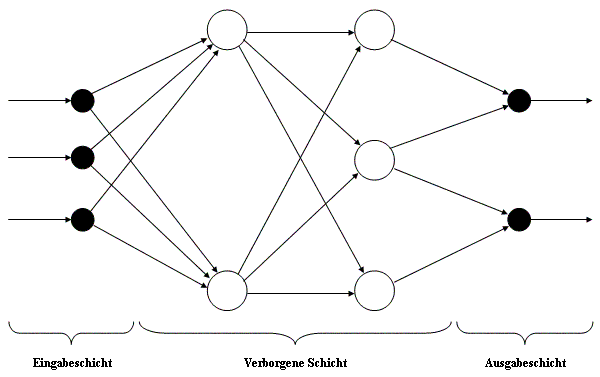
\includegraphics[width=10cm]{img/basic_neural_network}
  \caption{Schematische Darstellung eines neuronalen Netzwerkes. Links die Eingabeschicht, in der Mitte eine Hiddenschicht, rechts die Ausgabeschicht.}
  \label{fig:schichten}
\end{figure}

Über die Eingabeschicht treten die Eingabedaten $\mathbf{x} = (x_1, x_2, \dots, x_n)$ in das Netzwerk ein. Diese werden dann an die Neuronen der Hiddenschicht vorwärtspropagiert und diese berechnen damit ihre Aktivierungen. Diese Aktivierungen werden dann von der Hiddenschicht zur Ausgabeschicht weitergereicht wo die sich darin enthaltenen Neuronen wiederum ihre Aktivierung berechnen. Die Eingabewerte der einzelnen Neuronen der Ausgabeschicht sind dabei die Aktivierungen aller Neuronen der vorhergehenden Schicht. Eine solche Schicht wird auch als \emph{fully-conncted} Schicht bezeichnet. Dieser Vorgang des "Vorwärtsrechnens" wird auch als Vorwärtspropagierung bezeichnet. Bei einem neuronalen Netzwerk mit mehr als einer Hiddenschicht spricht man auch von einem \emph{Deep Neural Network}. Die Anzahl der Schichten und Neuronen in einem Neuronalen Netzwerk hängt von der konkreten Problemstellung ab.

\paragraph{Backpropagation mit Gradient-Descent} Wie bei fast allen Modelle des maschinellen Lernens, lernt das neuronale Netztwerk mittels dem Optimieren einer Fehlerfunktion. Das Optimieren dieser Fehlerfunktion wird im Normalfalls mittels dem \emph{Backpropagation}-Algorithmus in Verbindung mit \emph{Gradient-Descent} erzielt. Als Fehlerfunktion kann jede Funktion dienen, mit welcher der Aussagefehler des Netzwerks quanitifiziert werden kann. Als Beispiele können hier der $\operatorname{mse}(x) = $, MAE oder auch Categorical Cross-Entropy aufgeführt werden. Der Algorithmus kann in den folgenden Schritten zusammegefasst werden:

\begin{enumerate}
  \item Die Eingabewerte in das Netzwerk einführen und die Vorwärtspropagierung durchführen.
  \item Die Ausgabewerte des Netzwerks werden mit dem erwarteten Resultat vergleichen. Die Differenz der Ausgabewerte von den erwarteten Werten wird als Aussagefehler des Netzwerkes bezeichnet.
  \item Der Aussagefehler wird nun durch das neuronale Netzwerk hindurch zurückpropagiert. Dabei werden die Gewichte der einzelnen Schichten abhängig von ihrem Einfluss auf die berechneten Ausgangswerte verändert.
\end{enumerate}

Die Berechnung des Einfluss eines einzelnen Gewichtes wird mittels der partiellen Ableitung der Fehlerfunktion $E$ bezüglich dem entsprechenden Gewicht festgestellt. Danach wird das Gewicht neu berechnet indem man den Wert der partiellen Ableitung mal der Lernrate $\eta$ vom aktuellen Gewicht subtrahiert. Die Lernrate gibt dabei an wie stark sich ein einzelner Durchlauf von Backpropagation auf die Gewichte auswirken soll. Das neue Gewicht für das Neuron $i$ in der Schicht $k$ berechnet sich bei gegebener Lernrate $\eta$ und Fehlerfunktion $E$ also wie folgt:

\begin{equation}
w_{ik} = w_{ik} - \eta \frac{\delta E}{\delta w_{ik}}
\end{equation}

Gradient-Descent besitzt das Problem, dass der Erfolg des Algorithmus stark von der gewählten Lernrate $\eta$ abhängt. Bei einer zu grossen Lernrate wird das Optimum möglicherweise übersprungen oder der Werte der Fehlerfunktion divergiert sogar, bei einer zu kleinen Lernrate dauert es sehr lange bis das Optimum der Fehlerfunktion gefunden wird (vgl. Abbildung~\ref{fig:learn_rates}). Darum wird im Rahmen dieser Arbeit eine weiterentiwckelte Variante mit dem Namen \emph{AdaDelta} \cite{zeiler2012adadelta} verwendet. Diese hat den grossen Vorteil das keine Lernrate mehr definiert werden muss.

\begin{figure}[h]
  \centering
  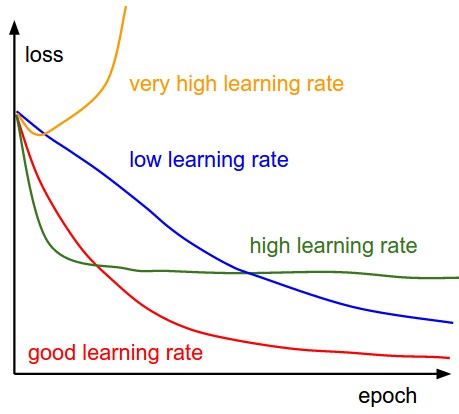
\includegraphics[width=6cm]{img/learning_rates_comparison}
  \caption{Beispielhafte gegenüberstellung verschiedener Lernraten\protect\footnote{http://cs231n.github.io/assets/nn3/learningrates.jpeg}}
  \label{fig:learn_rates}
\end{figure}

\section{Convolutional Neural Network}
\emph{Convolutional Neural Networks}, abgekürzt \gls{cnn}, sind eine spezielle Form der zuvor beschriebenen Neuronalen Netzen. Der grundlegende Unterschied besteht darin, dass die einzelnen Schichten nicht fully-conntected sind, sondern mittels Filter über lokale Konnektivität versucht wird Muster zu erkennen. Im folgenden werden die einzelnen Komponenten des in dieser Arbeit verwendeten CNNs erläutert.

\paragraph{Filter}\label{basic:cnn:filter} Anstatt Neuronen wie im klassischen Neuronalen Netzwerk lernt eine CNN über die sogenannten Filter. Dabei handelt es sich um $n\times m$-Matrizen, welche Gewichte enthalten, analog zu den Gewichten der eingehenden Verbindungen bei Neuronen. Dabei werden die Filter-Matrizen über die Eingabedaten bewegt und es wird jeweils das innere Produkt der aktuellen Filter-Matrix und dem aktuellen Ausschnitt der Eingabedaten berechnet auf welchem der Filter positioniert ist. Das Bewegungsmuster des Filters wird \emph{Stride} (dt. durchschreiten) genannt. Im Rahmen dieser Arbeit wird nur ein eindimensionaler Stride entlang der Satz-Matrix (vgl. \ref{missing!}) verwendet.

Die durch diese Convolution-Operation resultierende Werte werden der Form einer Resultat-Matrix, der sogenannten \emph{Feature Map}, zwischengespeichert. Diese stellen also das Äquivalent zur Aktivierung einer Schicht im klassischen Neuronalen Netzwerk dar. Dabei werden alle resultierenden Feature-Maps einfach hintereinandergereiht und dienen als Eingabewerte für die nächste Schicht. 

\begin{figure}[h]
	\centering
	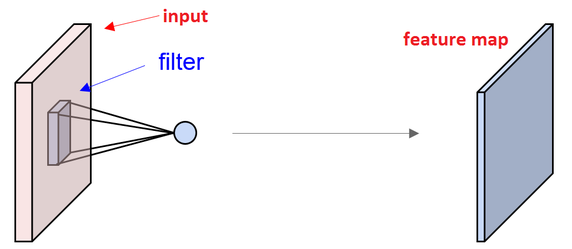
\includegraphics[width=10cm]{img/filter_feature_map}
	\caption{Schematische Darstellung Filter und Feature-Map}
\end{figure}

Eine Schicht, welche diese Art von Berechnung verwendet wird auch Convolutional (dt. fallten) Schicht genannt.

\paragraph{Max-Pooling Schicht} In der \emph{Max-Pooling} Schicht wird ein grossteil der in den Feature-Maps vorhandenen Informationen verworfen. Dabei wird ein Fenster über die resultierenden Feature-Maps der vorhergehenden Schicht bewegt und der jeweils maximale Wert des entsprechenden Ausschnitts der aktuellen Feature-Map als Wert in die gepoolte Represäntation übernommen. Das Fenster, welches über die Feature-Map bewegt wird, ist definiert durch die Dimensionalität des Fensters und dem Stride. Der Stride steht für das Bewegunsmuster des Fenster analog zum Filter. Die gepoolten Represäntationen der Feature-Maps dienen dann als Eingabewerte für die nächste Convolutional oder Ausgabeschicht.

\begin{figure}[H]
	\centering
	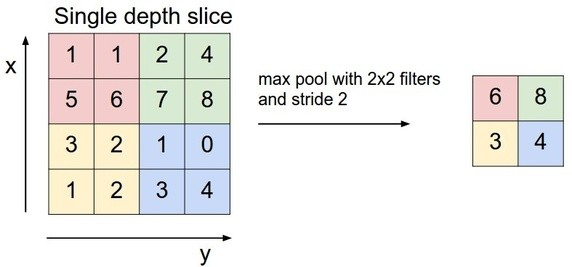
\includegraphics[width=10cm]{img/max_pooling}
	\caption{Schematische Funktionsweise der Max-Pooling Schicht}
\end{figure}

Die Max-Pooling Schicht erfüllt zwei Aufgaben: Einerseits reduziert sie die Dimensionalität der zu verarbeitenden Daten, andererseits verwirft sie \quotes{unwichtige} Informationen indem sie nur die maximalen Werte der zuletzt berechneten Aktivierungen behält.\fixme{more infos?}

\paragraph{Convolutional+Max-Pooling Schicht} Die Convolutional und Max-Pooling Schicht bilden die Grundbausteine des CNN. Diese werden nun mehrfach hintereinander gereiht. Das im Rahmen dieser Arbeit vewendete CNN hat bespielsweise zwei solcher aufeinanderfolgenden Convolutional+Max-Pooling Schichten.

\begin{figure}[h]
	\centering
	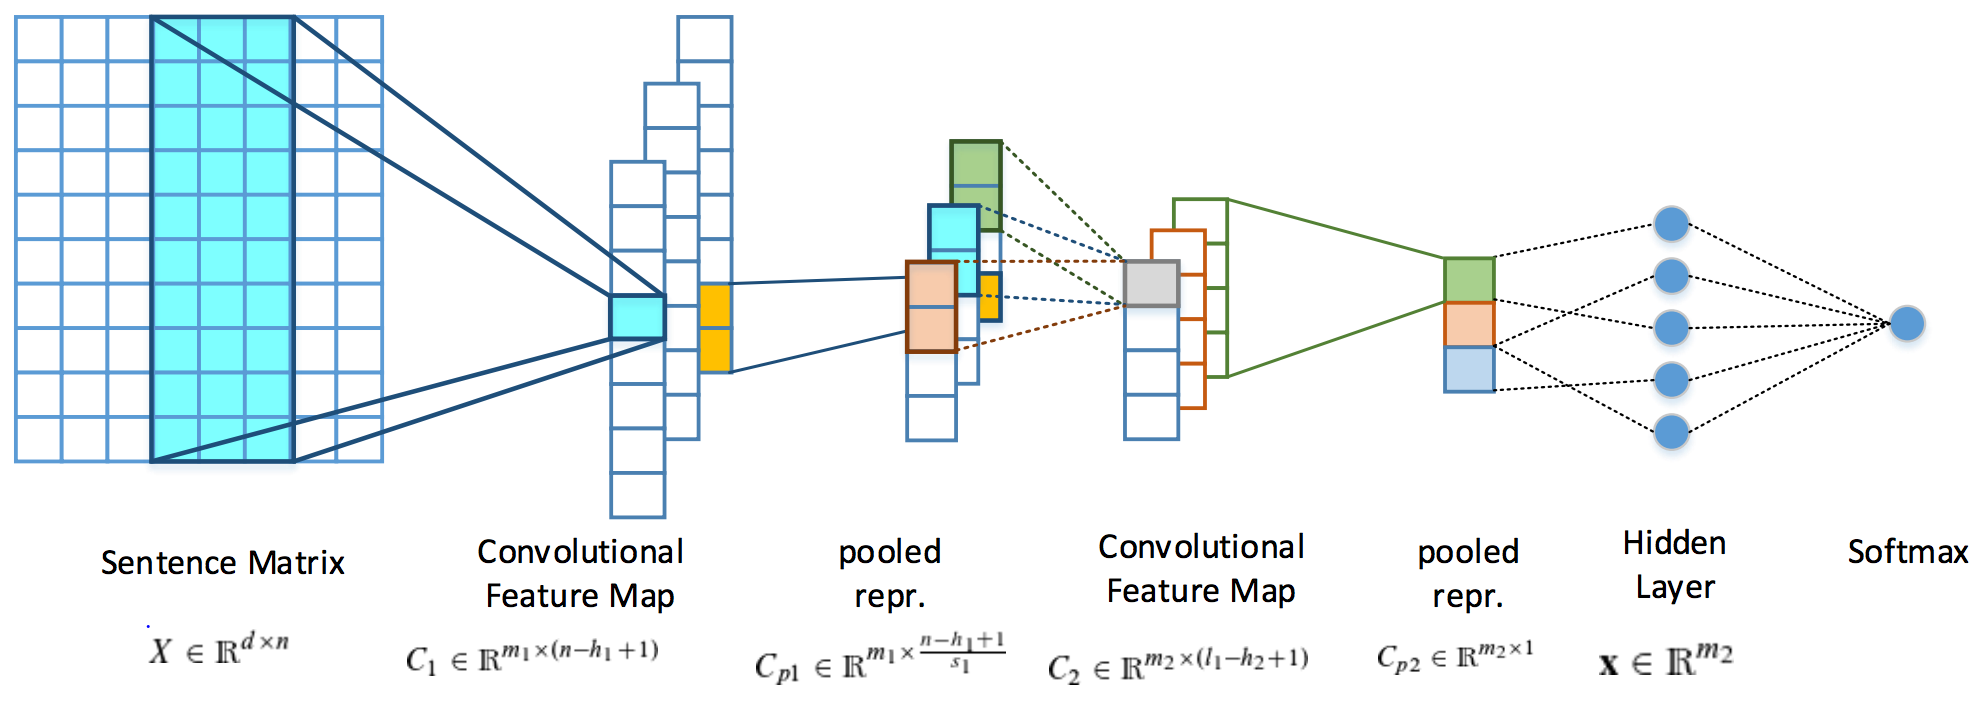
\includegraphics[width=10cm]{img/semeval_cnn_structure}
	\caption{Schematische Darstellung des in dieser Arbeit verwendeten CNN \protect\cite{deriu2016swisscheese}}
\end{figure}

\paragraph{Ausgabeschicht}\label{basic:cnn:output_layer} Die Ausgabeschicht des CNN ist gleich aufgebaut wie die eines \quotes{traditionellen} Neuronalen Netzwerks. Dabei wird eine fully-connected Schicht verwendet bei welcher alle Neuronen als Eingabewerte alle Aktivierungen der letzten Max-Pooling Schicht verknüpft sind. Die Anzahl Neuronen entspricht dabei der Anzahl zu unterscheidenden Klassen.

\section{3-Phasen Lernen}

Das Training des CNNs wird mithilfe des 3-stufigen Lernverfahren von Severyn et. al. \cite{Severyn:2015kta} durchgeführt. Im Folgenden werden die einzelnen Schritte im Detail erläutert.

\paragraph{Word-Embeddings und Satz-Matrix} Zuerst werden mithilfe von \emph{word2vec}~\cite{mikolov2013distributed} und einem grossen Text-Corpus Word-Embeddings generiert. Dabei werden die gegebenen Wörter eines Vokabulars $v$ so in einen reelen Vektorraum $\mathbb{R}^d$ abgebildet, dass die semantischen Beziehungen innerhalb der Wörter erhalten bleiben. Dies wird am Beispiel in Abbildung \ref{fig:king_queen_example} ersichtlich: Die Wortvektoren für \quotes{Man} and \quotes{Woman} stehen in gleicher Weise zueinander wie die Wortvektoren \quotes{Uncle} zu \quotes{Aunt} bzw. \quotes{King} zu \quotes{Queen}.

\begin{figure}[H]
  \label{fig:king_queen_example}
  \centering
  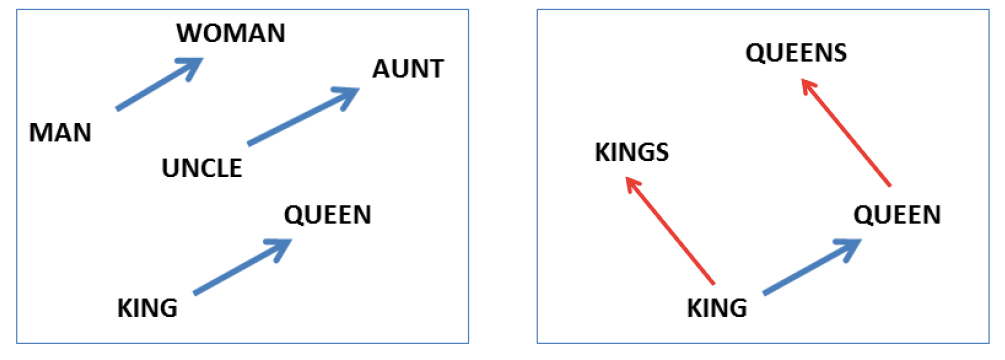
\includegraphics[width=10cm]{img/king_queen_example_word_embeddings}
  \caption{Beispiel für semantische Beziehung von Wort-Vektoren}
\end{figure}

Mithilfe der Word-Embeddings kann ein gegebener Satz nun als Konkatenation der Vektoren der einzelnen Wörter aufgefasst werden. Das bedeutet, dass ein Satz als $d \times n$ Matrix dargestellt werden kann, wenn $n$ die Anzahl Wörter des Satzes darstellt und $d$ die Anzahl Dimensionen der Word-Embeddings. Die $i$-te Zeile in der resultierenden Satz-Matrix entspricht dann dem Wort-Vektor für das $i$-te Wort im abzubildenden Satz.

\paragraph{Distant-Supervision Phase} In einem zweiten Schritt wird die sogenannte \emph{Distant-Supervised} Phase durchgeführt. Dabei wird das CNN mit einer grossen Menge an \emph{weakly-labeled} (dt. schwach annotiert) Texten über eine Epoche hinweg vortrainiert. Weakly labeled bedeutet, dass der Sentiment eines Textes aus der Eigenschaft des Textes abgeleitet wird und nicht von Hand annotiert wurde. Beispiele für Eigenschaften, aus welchen sich ein Sentiment ableiten lässt sind Emoticons in Tweets oder die Anzahl der vergebenen Sterne bei einer Produktbewertung. Bei Emoticons lässt sich zum Beispiel aus dem lachenden Emoticon \quotes{:-)} ein positiver bzw. aus dem traurigen Emoticon \quotes{:-(} ein negativer Sentiment ableiten.\fixme{more informations on how the distant phase works in our case!}

% Wie bereits in \ref{basics:neural_network} erläutert benötigen NNs, vor allem CNNs, sehr viele annotierte Trainingsdaten \fixme{Referenz} um am Ende des Trainings ein zufriedenstellendes Modell zu erhalten. Ein grossteil der vorhandenen Datensätze umfassen allerdings nicht mehr als 10'000 Texte. Des Weiteren sind die Sentiments in diesen Datensätzen sehr oft nicht gleichverteilt. Das führt dazu, dass gewisse Sentiments unterrepräsentiert sind, während andere überdurchschnittlich oft vorhanden sind. Im Falle der in dieser Arbeit verwendeten Datensätze ist es so, dass der positive und negative Sentiment unterdurchschnittlich oft vorkommen, während es überdurchschnittlich viele Texte mit einem neutralen Sentiment gibt (vgl. \ref{data:supervised_data}). Dadurch lernt das CNN zwar sehr gut Texte mit neutralem Sentiment zu erkennen, allerdings tut es sich sehr schwer mit den anderen beiden Sentiments.

% Um dieses Problem zu beheben kann das Training mit sogenannter \emph{Distant Supervision} \cite{} durchgeführt werden. Die Grundidee dabei ist einen grossen, unsupervised Corpus an Trainingsdaten zu verwenden bei welchem sich der Sentiment eines einzelnen Datensatzes aus einer Eigenschaft des Datensatzes ableiten lässt. Beispiele für Eigenschaften aus welchen sich der Sentiment ableiten lässt sind zum Beispiel Emoticons in Tweets oder die Anzahl der vergebenen Sterne bei einer Produktbewertung auf Amazon aufführen. Bei den Emoticons in Tweets lässt sich so zum Beispiel aus dem lachenden Emoticon \quotes{:-)} ein positiver bzw. aus dem traurigen Emoticon \quotes{:-(} ein negativer Sentiment ableiten. Erläuterungen wie die Distant Supervision im Rahmen dieser Arbeit verwendet wurde wird im Kapitel Methodik genauer erläutert (vgl. \ref{methods:distant_supervision}).

\paragraph{Supervised Phase} Im letzten Schritt wird das CNN mit den von Hand annotierten Texten trainiert. Dieses Training wird mithilfe von Backpropagation mit AdaDelta durchgeführt. Dabei wird sogenanntes \emph{Early Stopping verwendet}: Das Netzwerk wird solange trainiert, bis eine definierte Metrik über eine bestimmte Anzahl Epochen nicht mehr verbessert hat.

\section{Evaluierungsmetrik}
Im folgenden wird die verwendete Evaluierungsmetrik, der \emph{F1-Score}, erläutert.

\paragraph{Precision {\&} Recall} \emph{Precision} (dt. Präzision) und \emph{Recall} (dt. Ausbeute) sind Metriken, mit welchen die Performanz eines Systems evaluiert werden kann. Dabei ist die Precision das Verhältnis von richtig klassifizierten ($tp$) zu allen klassifizierten Samples ($tp + fp$):
\begin{equation}
precision = \frac{tp}{tp + fp}
\end{equation}
Die Ausbeute ist das Verhältnis von richtig klassifizierten zur Anzahl aller vorhandenen Samples ($tp + fp$).
\begin{equation}
recall = \frac{tp}{tp + fp}
\end{equation}
\paragraph{F1-Score} Um da oben beschriebene Problem zu lösen wird der F1-Score verwendet. Dieser ist das harmonische Mittel von Präzision und Ausbeute:
\begin{equation}
\label{basic:metrics:f1_eq}
F1 = \frac{2 \times precision \times recall}{precision + recall}
\end{equation}
Durch diese Metrik kann die Performanz eines Systems mittels eines Wertes quantifiziert werden. Ausserdem löst diese das Problem, dass eine hohe Präzision bzw. Ausbeute erzielt werden kann, wenn das System \quotes{schummelt} indem dieses immer die am stärksten vertretene Klasse als Antwort liefert.
\paragraph{F1-Score über mehrere Klassen} Der F1-Score selbst kann nur jeweils für eine einzelne Klasse bestimmt werden. Um nun aber eine einzige Metrik für die Messung der Performanz des Systems über mehrere Klassen hinweg zu erhalten, werden die F1-Scores der einzelnen Klassen summiert und durch die Anzahl der Klassen dividiert. Durch diese Vorgehen erhält man folgende Gleichung, wobei $k_i$ für eine einzelnen Klasse und $n$ für die Anzahl der beachteten Klassen:
\begin{equation}
\operatorname{F1}_{k_0, k_1, \dots, k_n} = \frac{\sum_{i=0}^{n} \operatorname{F1}_{k_i}}{n}
\end{equation}
Diese Art des F1-Score wird auch "makro" F1-Score genannt.

% \subsection{Präzision {\&} Ausbeute}
% \label{basics:metrics:precision_recall}

% \subsection{F1-Score}
% Die in \ref{basics:metrics:precision_recall} beschriebenen Metriken Präzision und Ausbeute haben ein fundamentales Problem: Wenn die Klassen ungleich verteilt sind kann eine hohe Präzision bzw. Ausbeute erreicht werden indem einfach immer die am stärksten vertretene als Resultat zurückgegeben wird.

% Am Beispiel der Testdaten aus den JCR{\_}quotations (vgl. \ref{data:supervised_data}) ist einfach ersichtlich wo das Problem liegt. Der neutrale Sentiment ist hier überdurchschnittlich hoch vertreten mit $66.9\%$. Wenn der Klassifizierer also immer also Resultat den neutralen Sentiment zurückgibt führt das automatisch zu einer Ausbeute von $100\%$ und einer Präzision von $66.9\%$. Dies entspricht zwar der Realität ist aber irreführend.

% Um dieses Problem zu umgehen wird im Rahmen dieser Arbeit der F1-Score verwendet. Diese wird als Kombination der Präzision und der Ausbeute mithilfe der Gleichung \ref{basic:metrics:f1_eq} berechnet.

% \begin{equation}
% \label{basic:metrics:f1_eq}
% F1 = \frac{2*precision*recall}{precision + recall}
% \end{equation}

% Der zusammengefasste F1-Score über die zwei Klassen $x$ und $y$ wird mithilfe der Gleichung \ref{basic:metrics:f1_comb_eq} berechnet.

% \begin{equation}
% \label{basic:metrics:f1_comb_eq}
% F1_{x|y} = \frac{F1_x + F1_y}{2}
% \end{equation}

\section{Technischer Aufbau}
Im folgenden Abschnitt wird der technische Aufbau, welcher verwendet wurde, um die in \ref{experiments} beschriebenen Experimente durchzuführen.

\subsection{Vorarbeiten}
\label{technichal_setup:prework}
Der Grundaufbau der verwendeten Software wurde vom InIT mithilfe von Keras\footnote{https://keras.io/} implementiert und zur Durchführung dieser Arbeit zur Verfügung gestellt. Im Rahmen dieses Grundaufbaus wurde die folgende Funktionalität bereits implementiert:

\begin{itemize}[noitemsep]
	\item Implementation des CNN in Keras und verwendung von Theano \cite{theanoCitShort} als Backend für die GPUs (vgl. Abschnitt \ref{technichal_setup:hardware}).
	\item Implementation von Evaluations-Metriken
	\item Skripte mit den folgenden Funktionalitäten: Trainieren des CNN, Laden von TSV Dateien, Vorverarbeiten von Word-Embeddings
\end{itemize}

\subsection{Anforderungen}
\label{technical_setup:requirements}
Ein System, welches die in \ref{experiments} beschriebenen Experimente durchführen kann, soll die folgenden Eigenschaften aufweisen:

\begin{itemize}
	\item \textbf{Parametrisierbarkeit}: Dadurch dass eine grosse Anzahl kleiner Experimente durchgeführt werden muss soll das System die Möglichkeit bitten Experimente parametrisiert durchzuführen.
	\item \textbf{Wiederholbarkeit}: Experimente sollen wenn nötig mehrfach durchgeführt werden ohne einen Mehraufwand zu verursachen. 
	\item \textbf{Übersichtlichkeit}: Resultate der Experimente sollen übersichtlich und einfach zugänglich sein.
	\item \textbf{Auswertbarkeit}: Resultate sollen \fixme{Bessers Wort für Einfach?} einfach ausgewertet werden können.
\end{itemize}

Die in \ref{technichal_setup:prework} beschriebenen Vorarbeiten bitten eine Basis um damit ein System aufzubauen, welches die oben beschriebenen Eigenschaften aufweist.
\subsection{Funktionalität}
\label{technical_setup:functionality}
Um ein System, welches die im vorhergehenden Kapitel beschriebenen Eigenschaften aufweist, zu erhalten, wurden die folgenden Komponenten implementiert:

\begin{itemize}
	\item \textbf{Executor}: Der \emph{Executor} ist zuständig für das Training der CNNs mithilfe von Keras. Beim Start akzeptiert er die Konfiguration als Parameter. Das Experiment wird mit dem Laden der benötigten Daten und dem anschliessenden Training des CNN gestartet. Am Ende jeder Epoche wird das aktuelle CNN auf den Validierungsdaten getestet und die konfigurierten Metriken ausgewertet. Diese werden am Ende zusammen mit dem trainierten CNN (Gewichte im HDF5-Format\footnote{https://support.hdfgroup.org/HDF5/}, das CNN Model als JSON) in einen für das Experiment vorgesehenen Ordner gespeichert. Die Metriken werden ebenfalls in diesem dem dafür vorgesehenen Ordner abgespeichert.
	\item \textbf{Config Management}: Experimente werden über Konfigurationen im JSON-Format\footnote{http://www.json.org/} parametrisiert. Über diese Konfiguration können viele wichtige Parameter für die Ausführung festgelegt werden, so zum Beispiel: Anzahl Epochen, Trainings- und Validierungsdaten, Parameter für k-fold Cross-Validation oder auch bereits Trainierte Modelle können geladen werden. Für eine vollständige Liste wird auf den Quellcode des Projektes verwiesen. Experimente können mittels der group{\_}id gruppiert werden. Damit können die Experimente hierarchisch mittels zwei Ebenen gruppiert werden.
	\item \textbf{DataLoader}: Mithilfe des \emph{DataLoader} können Trainings- und Validierungsdaten im TSV\footnote{https://reference.wolfram.com/language/ref/format/TSV.html} Dateiformat geladen werden. Die zu ladenden Daten können dabei aus einer oder mehreren TSV-Dateien stammen. Im Falle das mehrere TSV Dateien angegeben werden kann über die Konfiguration das Verhältnis angegeben werden, in welchem die Daten aus den einzelnen Dateien verschmischt werden sollen.
	\item \textbf{Skripte}: Die Auswertung der einzelnen Experimente geschieht über dafür erstelle Skripte (vgl. \ref{technical_setup:scripts}).
	\item \textbf{Weboberfläche}: Auf die Resultate der Experimente können über eine eigens dafür entwickelte Weboberfläche zugegriffen werden. Ausserdem besteht die Möglichkeit Plots über die Metriken welche während des Trainings- und Validierungsprozess gesammelt wurden auszuwerten (vgl. \ref{technical_setup:webgui}).
\end{itemize}
\fixme{Referenze auf Code, Code-Style bei group{\_}id}
Die oben beschriebenen Komponenten erlauben es Experimente mittels JSON Konfigurationen zu starten und den gesamten Trainings- und Validierungsprozess mittels der Metriken zu dokumentieren.

\subsection{Skripte}
\label{technical_setup:scripts}
Für die Durchführung der Experimente wurden diverse Skripte erstellt um die Handhabung zu vereinfachen und Auswertungen zu ermöglichen. Die Liste der implementierten Script umfasst unter anderem die folgenden:

\begin{itemize}[noitemsep]
	\item Erstellen von Plots der Lernkurven und Metriken
	\item Erstellen von Word-Embeddings über einen Textcorpus
	\item Erstellen von Statistiken zu Trainings- und Validierungsdaten
	\item Vorverarbeitung von Trainingsdaten für die Distant-Phase
	\item Erstellen von Visualisierungen von Word-Embeddings mittels t-SNE \cite{maaten2008visualizing}
	\item Diverse Wartungsscripkte zur Generierung und Verwaltung von Experimenten
\end{itemize}

\subsection{Weboberfläche}
\label{technical_setup:webgui}
Um die dritte Anforderung nach Übersichtlichkeit und Auswertbarkeit (vgl. \ref{technical_setup:requirements}) zu erfüllen wurde eine Weboberfläche umgesetzt, mit welchem die Parameter und Resultate aller durchgeführten Experimente übersichtlich und an einem Ort zur Verfügung gestellt werden. Für die Implementation wurde das Python Framework flask\footnote{http://flask.pocoo.org/} verwendet.\fixme{Bilder der Weboberfläche, Schrift flask}

Zur Auswertung der Experimente stehen drei Funktionen zur Verfügung:
\begin{itemize}
	\item Die Oberfläche gewährt Zugriff auf alle JSON Konfigurationen, welche zu einem Experiment gehören. Dazu zählen die Konfiguration selbst, die gespeicherten Trainings- und Validierungsmetriken und das CNN Model (vgl. \ref{technical_setup:functionality}).
	\item Mittels der Plotting Funktion können Plots von Trainingsmetriken erstellt werden. Weiterhin können Plots und Boxplots über die die Validierungsmetriken der einzelnen Schritte der Crossdomain-Experimente (vgl. \ref{methods:v8}) erstellt werden.
	\item Die gespeicherten Validierungs- und Trainingsmetriken können mithilfe von math.js\footnote{http://mathjs.org/} direkt im Browser ausgewertet werden.\fixme{Code-Style}
\end{itemize}
\begin{figure}[htbp]
	\centering
	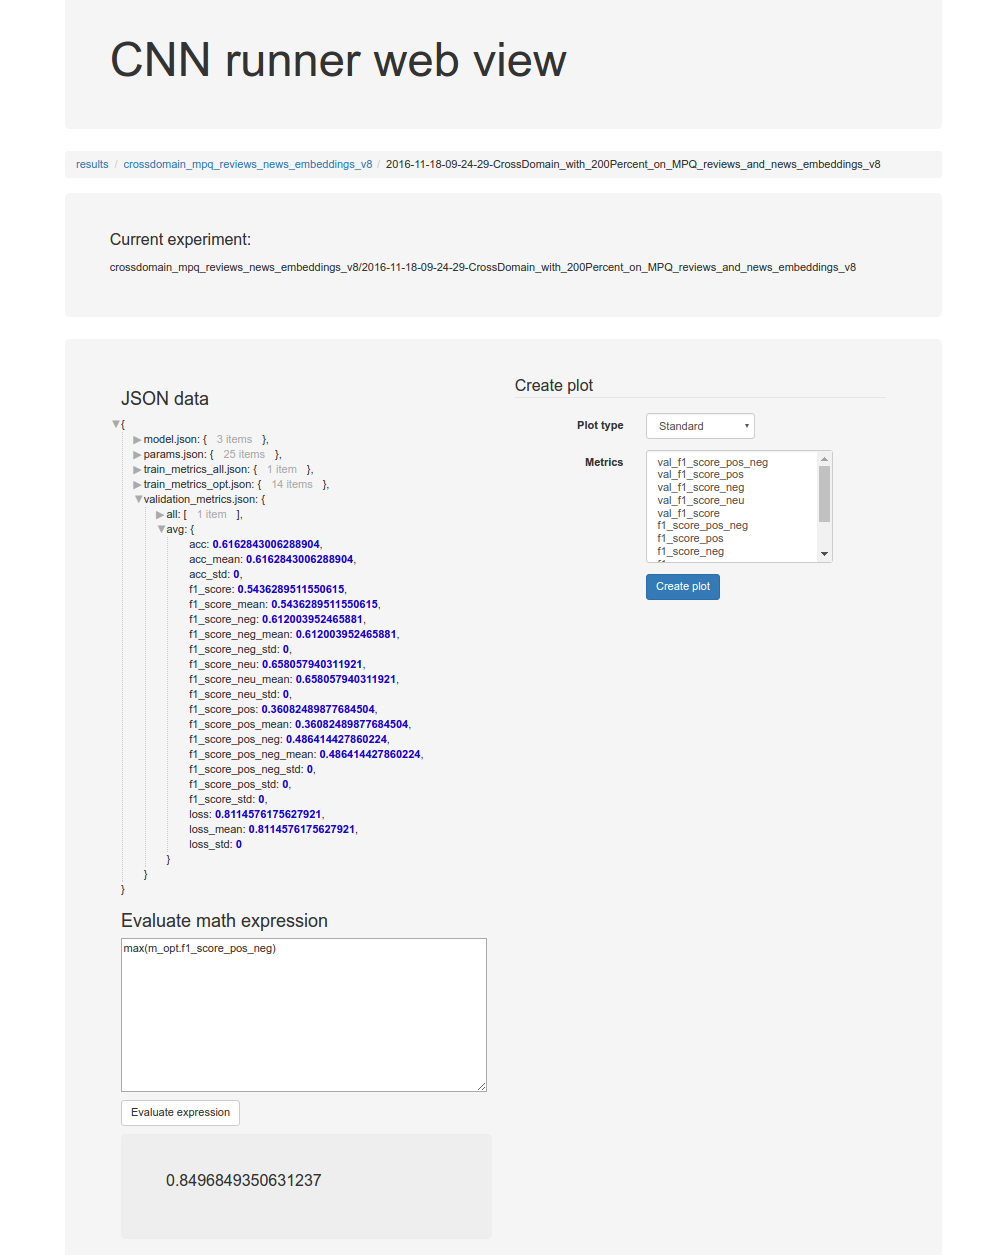
\includegraphics[width=0.7\textwidth]{img/web_gui}
	\caption{Ansicht Experiment über Weboberfläche}
	\label{fig:web_gui}
\end{figure}
\subsection{Betriebssystem \& Softwarepakete}
\label{technical_setup:software}
Alle Experimente wurden mit der unten beschriebenen Implementation durchgeführt. Auf beiden verwendeten Computer-Systemen (vgl. \ref{technichal_setup:prework}) wurde als Betriebssystem Ubuntu 16.04 installiert. Dazu wurden Python 3.5.2\footnote{https://www.python.org/}, Nvidia GPU Treiber und cuda8\footnote{https://developer.nvidia.com/cuda-toolkit} als Abhängigkeiten von Theano und Keras installiert.

\subsection{Hardware}
\label{technichal_setup:hardware}
Zur Durchführung der Experimente wurden zwei unterschiedliche Computer verwendet. Im ersten System (S1) ist eine Nvidia GTX970 GPU, einen Intel i7 4950K CPU und 16GB Arbeitsspeicher installiert. Das zweite System besitzt eine Nvidia GTX1070 GPU, einen Intel i7 6700K CPU und ebenfalls 16GB Arbeitsspeicher. Die Unterschiede in der Hardware haben keinen Einfluss auf die Experimente, da auf beiden System dasselbe Betriebssystem mit den gleichen Softwarepaketen verwendet wurde (vgl. \ref{technical_setup:software}).

